\documentclass[12pt, a4paper]{article}

\usepackage{amsmath} 
\usepackage[margin=1in]{geometry}
\usepackage{tikz}
\usetikzlibrary{
  shapes.geometric,
  arrows.meta,
  positioning,
  fit,
  backgrounds,
  calc,
  decorations.pathreplacing
}
\usepackage{xcolor}
\usepackage{float}
\usepackage{caption}

% ── Colour palette ────────────────────────────────────────────────────────────
\definecolor{asrblue}  {RGB}{41,  128, 185}
\definecolor{llmgreen} {RGB}{39,  174,  96}
\definecolor{ttsred}   {RGB}{192,  57,  43}
\definecolor{uipurple} {RGB}{142,  68, 173}
\definecolor{storegold}{RGB}{243, 156,  18}
\definecolor{iocolor}  {RGB}{127, 140, 141}

% ── Shared TikZ styles ────────────────────────────────────────────────────────
\tikzset{
  svc/.style={
    draw=#1, fill=#1!10, rounded corners=5pt,
    minimum width=3.8cm, minimum height=3.2cm,
    align=center, thick, font=\small, text width=3.4cm
  },
  frontend/.style={
    draw=uipurple, fill=uipurple!10, rounded corners=6pt,
    minimum width=13cm, minimum height=1.6cm,
    align=center, thick, font=\small
  },
  storage/.style={
    draw=storegold!80!black, fill=storegold!10,
    rounded corners=4pt, dashed, thick,
    minimum width=13cm, minimum height=1.3cm,
    align=center, font=\small
  },
  ionode/.style={
    draw=iocolor, fill=iocolor!15, rounded corners=20pt,
    minimum width=2.0cm, minimum height=0.95cm,
    align=center, font=\small, thick
  },
  procbox/.style={
    draw=#1, fill=#1!12, rounded corners=5pt, thick,
    minimum width=3.0cm, minimum height=2.0cm,
    align=center, font=\small
  },
  databox/.style={
    draw=black!40, fill=white, rounded corners=2pt,
    inner sep=4pt, align=center, font=\scriptsize
  },
  latbox/.style={
    draw=black!25, fill=black!6, rounded corners=3pt,
    inner sep=4pt, align=center, font=\scriptsize
  },
}

\begin{document}

% ════════════════════════════════════════════════════════════════════════════════
% Figure 1 — System Architecture
% ════════════════════════════════════════════════════════════════════════════════
\begin{figure}[H]
\centering
\resizebox{\linewidth}{!}{%
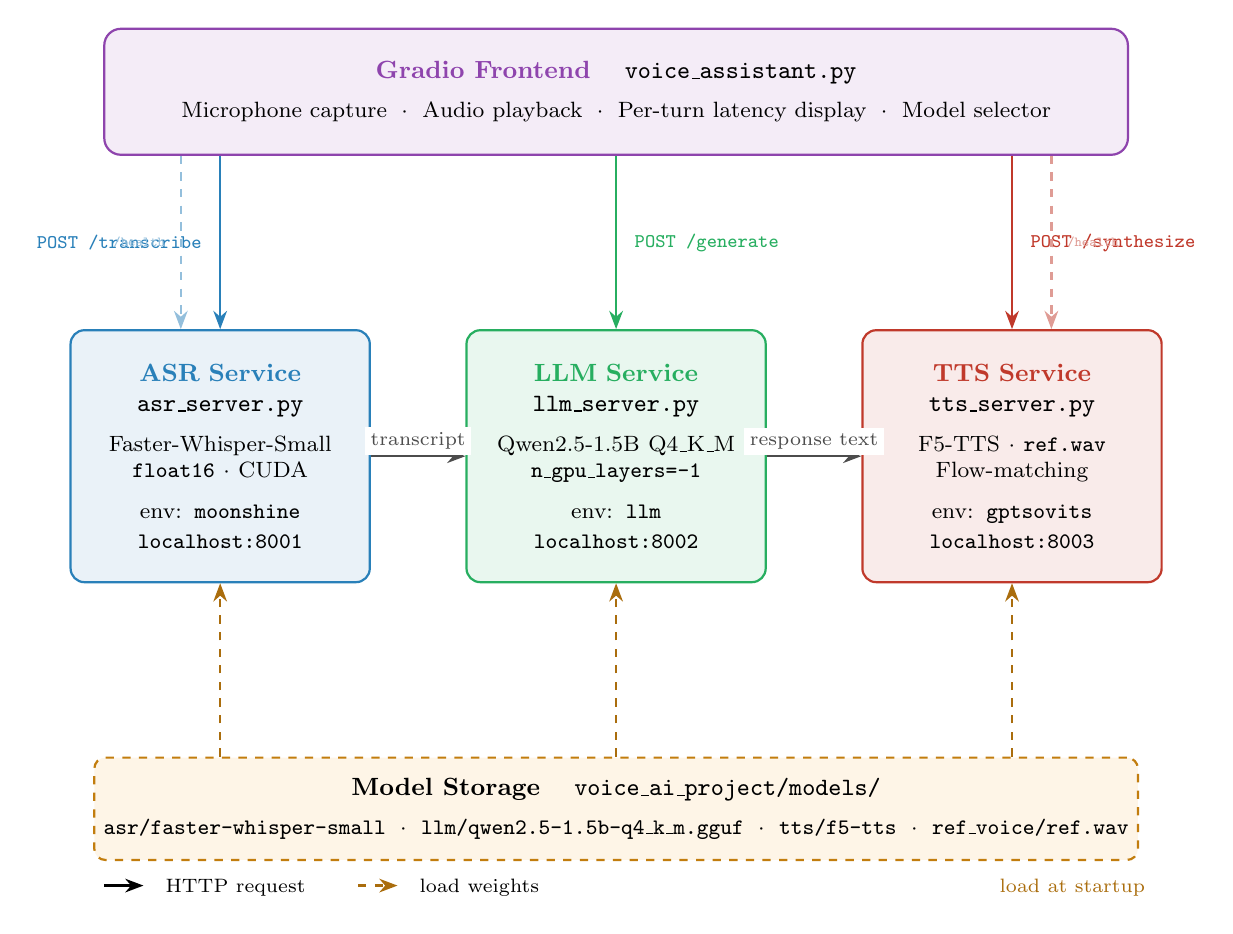
\begin{tikzpicture}[node distance=2.0cm]

% ── Gradio Frontend ───────────────────────────────────────────────────────────
\node[frontend] (fe) {
  \textbf{\color{uipurple}Gradio Frontend} \quad \texttt{voice\_assistant.py}\\[3pt]
  \footnotesize
  Microphone capture $\;\cdot\;$ Audio playback
  $\;\cdot\;$ Per-turn latency display $\;\cdot\;$ Model selector
};

% ── Three microservices ───────────────────────────────────────────────────────
% 修复点：以中心点(LLM)为基准，将其放在前端的正下方，再把ASR和TTS放在其左右两侧。
\node[svc=llmgreen, below=2.2cm of fe] (llm) {
  \textbf{\color{llmgreen}LLM Service}\\
  \texttt{llm\_server.py}\\[5pt]
  \footnotesize Qwen2.5-1.5B Q4\_K\_M\\
  \footnotesize \texttt{n\_gpu\_layers=-1}\\[5pt]
  \footnotesize env: \texttt{llm}\\
  \footnotesize \texttt{localhost:8002}
};

\node[svc=asrblue, left=1.2cm of llm] (asr) {
  \textbf{\color{asrblue}ASR Service}\\
  \texttt{asr\_server.py}\\[5pt]
  \footnotesize Faster-Whisper-Small\\
  \footnotesize \texttt{float16} $\cdot$ CUDA\\[5pt]
  \footnotesize env: \texttt{moonshine}\\
  \footnotesize \texttt{localhost:8001}
};

\node[svc=ttsred, right=1.2cm of llm] (tts) {
  \textbf{\color{ttsred}TTS Service}\\
  \texttt{tts\_server.py}\\[5pt]
  \footnotesize F5-TTS $\cdot$ \texttt{ref.wav}\\
  \footnotesize Flow-matching\\[5pt]
  \footnotesize env: \texttt{gptsovits}\\
  \footnotesize \texttt{localhost:8003}
};

% ── Arrows: frontend → services ───────────────────────────────────────────────
\draw[-Stealth, thick, asrblue]
  (fe.south -| asr.north) --
  node[left, font=\scriptsize, xshift=-3pt]{\texttt{POST /transcribe}}
  (asr.north);

\draw[-Stealth, thick, llmgreen]
  (fe.south) --
  node[right, font=\scriptsize, xshift=3pt]{\texttt{POST /generate}}
  (llm.north);

\draw[-Stealth, thick, ttsred]
  (fe.south -| tts.north) --
  node[right, font=\scriptsize, xshift=3pt]{\texttt{POST /synthesize}}
  (tts.north);

% ── Also show /health dashed ──────────────────────────────────────────────────
\draw[-Stealth, thick, dashed, asrblue!50]
  ($(fe.south -| asr.north)+(-0.5,0)$) --
  node[left, font=\tiny, xshift=-2pt]{\texttt{/health}}
  ($(asr.north)+(-0.5,0)$);

\draw[-Stealth, thick, dashed, ttsred!50]
  ($(fe.south -| tts.north)+(0.5,0)$) --
  node[right, font=\tiny, xshift=2pt]{\texttt{/health}}
  ($(tts.north)+(0.5,0)$);

% ── Arrows: services → services (pipeline flow) ───────────────────────────────
\draw[-Stealth, thick, black!70]
  (asr.east) --
  node[above, font=\scriptsize, fill=white, inner sep=2pt]{transcript}
  (llm.west);

\draw[-Stealth, thick, black!70]
  (llm.east) --
  node[above, font=\scriptsize, fill=white, inner sep=2pt]{response text}
  (tts.west);

% ── Model storage ─────────────────────────────────────────────────────────────
\node[storage, below=2.2cm of llm] (store) {
  \textbf{Model Storage} \quad \texttt{voice\_ai\_project/models/}\\[3pt]
  \footnotesize
  \texttt{asr/faster-whisper-small}
  $\;\cdot\;$ \texttt{llm/qwen2.5-1.5b-q4\_k\_m.gguf}
  $\;\cdot\;$ \texttt{tts/f5-tts}
  $\;\cdot\;$ \texttt{ref\_voice/ref.wav}
};

% ── Load arrows: storage → services ──────────────────────────────────────────
\draw[-Stealth, thick, dashed, storegold!70!black]
  (store.north -| asr.south) -- (asr.south);
\draw[-Stealth, thick, dashed, storegold!70!black]
  (store.north) -- (llm.south);
\draw[-Stealth, thick, dashed, storegold!70!black]
  (store.north -| tts.south) -- (tts.south);

% ── Load label ────────────────────────────────────────────────────────────────
\node[font=\scriptsize, color=storegold!70!black,
      below right=0.1cm and 0.2cm of store.south east, anchor=north east]
  {load at startup};

% ── Legend ────────────────────────────────────────────────────────────────────
\node[font=\scriptsize, align=left,
      below left=0.1cm and 0cm of store.south west, anchor=north west] {
  \tikz\draw[-Stealth,thick,black](0,0)--(0.5,0); \; HTTP request \qquad
  \tikz\draw[-Stealth,thick,dashed,storegold!70!black](0,0)--(0.5,0); \; load weights
};

\end{tikzpicture}
}% end resizebox
\caption{System architecture. Three FastAPI microservices run in isolated Conda environments and are
orchestrated sequentially by the Gradio front end. Each service exposes a \texttt{/health} liveness
endpoint and a dedicated inference endpoint. Model weights are loaded from shared storage at startup.}
\label{fig:architecture}
\end{figure}


% ════════════════════════════════════════════════════════════════════════════════
% Figure 2 — Data Flow
% ════════════════════════════════════════════════════════════════════════════════
\begin{figure}[H]
\centering
\resizebox{\linewidth}{!}{%
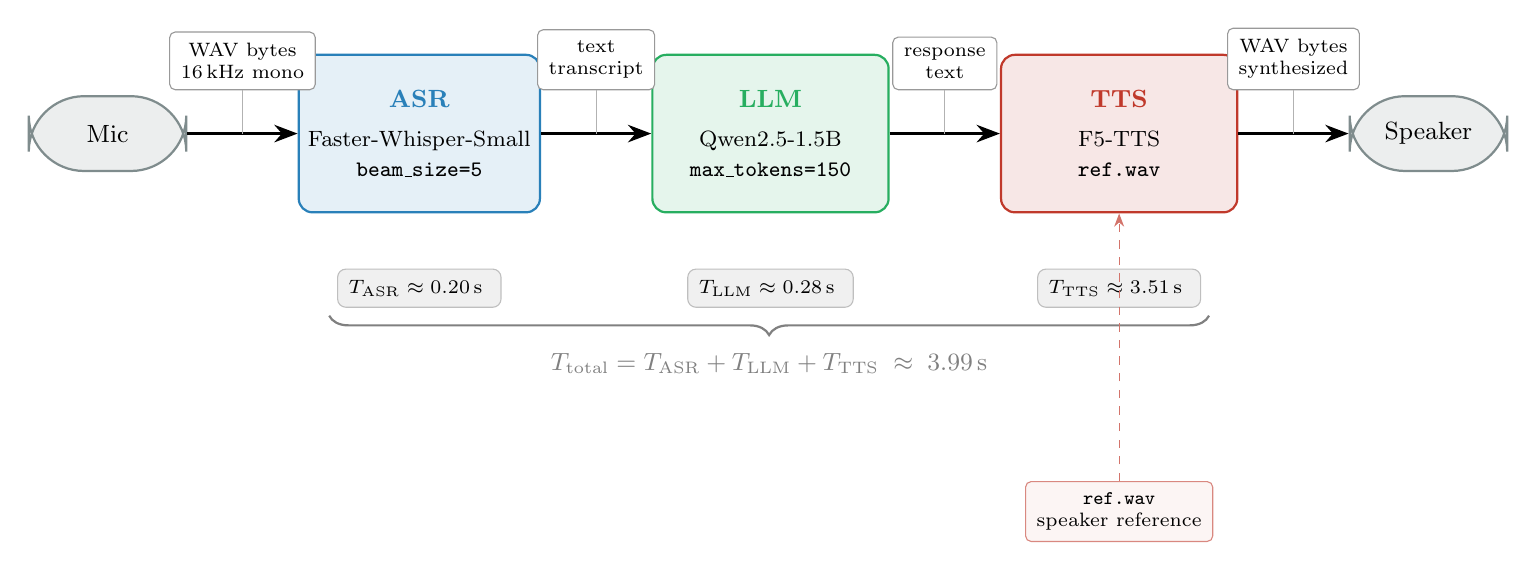
\begin{tikzpicture}[node distance=0pt]

% ── I/O nodes ─────────────────────────────────────────────────────────────────
\node[ionode] (mic) {Mic};

\node[procbox=asrblue, right=1.4cm of mic] (asrbox) {
  \textbf{\color{asrblue}ASR}\\[3pt]
  \footnotesize Faster-Whisper-Small\\
  \footnotesize \texttt{beam\_size=5}
};

\node[procbox=llmgreen, right=1.4cm of asrbox] (llmbox) {
  \textbf{\color{llmgreen}LLM}\\[3pt]
  \footnotesize Qwen2.5-1.5B\\
  \footnotesize \texttt{max\_tokens=150}
};

\node[procbox=ttsred, right=1.4cm of llmbox] (ttsbox) {
  \textbf{\color{ttsred}TTS}\\[3pt]
  \footnotesize F5-TTS\\
  \footnotesize \texttt{ref.wav}
};

\node[ionode, right=1.4cm of ttsbox] (spk) {Speaker};

% ── Main flow arrows ──────────────────────────────────────────────────────────
\draw[-Stealth, very thick] (mic)    -- (asrbox);
\draw[-Stealth, very thick] (asrbox) -- (llmbox);
\draw[-Stealth, very thick] (llmbox) -- (ttsbox);
\draw[-Stealth, very thick] (ttsbox) -- (spk);

% ── Data labels above arrows ──────────────────────────────────────────────────
\node[databox, above=0.55cm of $(mic.east)!0.5!(asrbox.west)$] (d1) {
  WAV bytes\\16\,kHz mono
};
\node[databox, above=0.55cm of $(asrbox.east)!0.5!(llmbox.west)$] (d2) {
  text\\transcript
};
\node[databox, above=0.55cm of $(llmbox.east)!0.5!(ttsbox.west)$] (d3) {
  response\\text
};
\node[databox, above=0.55cm of $(ttsbox.east)!0.5!(spk.west)$] (d4) {
  WAV bytes\\synthesized
};

% ── Connector lines to data labels ────────────────────────────────────────────
\draw[gray!60, thin] ($(mic.east)!0.5!(asrbox.west)+(0,0)$) -- (d1.south);
\draw[gray!60, thin] ($(asrbox.east)!0.5!(llmbox.west)$)    -- (d2.south);
\draw[gray!60, thin] ($(llmbox.east)!0.5!(ttsbox.west)$)    -- (d3.south);
\draw[gray!60, thin] ($(ttsbox.east)!0.5!(spk.west)$)       -- (d4.south);

% ── Latency boxes below ───────────────────────────────────────────────────────
\node[latbox, below=0.7cm of asrbox] (l1) {
  $T_{\text{ASR}} \approx 0.20$\,s
};
\node[latbox, below=0.7cm of llmbox] (l2) {
  $T_{\text{LLM}} \approx 0.28$\,s
};
\node[latbox, below=0.7cm of ttsbox] (l3) {
  $T_{\text{TTS}} \approx 3.51$\,s
};

% ── Brace spanning all three latency boxes ────────────────────────────────────
\draw[decorate,
      decoration={brace, amplitude=7pt, mirror},
      thick, black!50]
  ($(l1.south west)+(-0.1,-0.1)$) -- ($(l3.south east)+(0.1,-0.1)$)
  node[midway, below=10pt, font=\small]{
    $T_{\text{total}} = T_{\text{ASR}} + T_{\text{LLM}} + T_{\text{TTS}}
    \;\approx\; 3.99\,\text{s}$
  };

% ── Reference voice annotation ────────────────────────────────────────────────
\node[databox, below=0.7cm of ttsbox |- l3.south,
      yshift=-1.5cm, xshift=0cm,
      draw=ttsred!60, fill=ttsred!5,
      font=\scriptsize] (refwav) {
  \texttt{ref.wav}\\speaker reference
};
\draw[-Stealth, ttsred!70, dashed, thin]
  (refwav.north) -- (ttsbox.south);

\end{tikzpicture}
}% end resizebox
\caption{Data flow through the integrated pipeline. WAV audio from the microphone is transcribed by
the ASR service, forwarded as text to the LLM, and the generated response is synthesized to speech by
the TTS service using a fixed reference voice clip. Latency values are measured per-turn in the
integrated system (CUDA). The TTS stage dominates end-to-end latency at $\approx$88\%.}
\label{fig:dataflow}
\end{figure}

\end{document}